\section{Primzahlen}\label{Kapitel Primzahlen}
	Natürliche Primzahlen werden definiert durch Zahlen > 1 die nur durch Eins oder sich selbst teilbar sind. Wie im Kapitel Primfaktorzerlegung gezeigt, können alle natürlichen Zahlen mit einer Multiplikation von Primzahlen erzeugt werden. Sie bilden sozusagen die Bausteine aller natürlichen Zahlen. Die Unberechenbarkeit mit der sie auftreten gibt Mathematikern schon seit Jahrtausenden Rätsel auf und ist ein Grundstein unserer heutigen Verschlüsselungsverfahren.
	In anderen Zahlensystemen als den natürlichen Zahlen ist die gewohnte Definition von Primzahlen nicht vollständig/korrekt. Sie sagt nur etwas über die Irreduzibelität eines Elements in einem Integritätsbereich aus. Da in den natürlichen Zahlen aber jedes irreduzibles Element auch prim ist reicht diese Definition für \myMenge{N} aus.
	Für alle Integritätsbereiche gilt für die Primheit folgende Definition nach \cite{Algorithmische:Zahlentheorie}:
	
	Ein Element \myMathRM{p \in R\setminus(R^* \cup~\{0\})} heißt prim oder Primelement, wenn für alle \myMathRM{a, b \in R\setminus\{0\}} gilt:	
	\begin{displaymath}
		p~|~ab \Longrightarrow p~|~a~oder~p~|~b.
	\end{displaymath}
		
	Mit Hilfe der Primzahlen kann der Restklassenring \myMenge{Z}/m\myMenge{Z} spezialisiert werden. Ist m eine Primzahl p, so ist \myMenge{Z}/p\myMenge{Z} ein Körper und wird auch \myMenge{F}\myTiefstellen{p} bzw. \myMenge{GF}\myTiefstellen{p} bezeichnet.
	
	Neben den normalen Primzahlen gibt es weitere sogenannte Pseudoprimzahlen. Diese Primzahlen verhalten sich bezogen auf einen Algorithmus genauso wie echte Primzahlen, sie sind jedoch zusammengesetzt. Ein Beispiel für solche Zahlen sind Carmichaelzahlen die in einem späteren Kapitel thematisiert sind.

	Leider gibt es keine bekannten effizienten Verfahren um Primzahlen zu generieren. Dennoch kann man Primzahlen recht einfach raten. Grundsätzlich ist es möglich eine große Anzahl von Zahlen auszuschließen. Man denke an: nur ungerade Zahlen, die Teilungsgesetze und die Tatsache das alle Primzahlen > 3 in der Form 4k +1 oder 4k +3, k \myin \myMenge{N} vorliegen. Alle geratenen Zahlen müssen jedoch einem Primzahltest(vgl. Kapitel \ref{Effiziente Primzahltests}) zur Verifizierung unterzogen werden. In \cite{Algebraische:und:zahlentheoretische:Grundlagen:fuer:die:Informatik} ist beschrieben wie ein Generierungsprozess erfolgen kann.

	\subsection{Primfaktorzerlegung}
	Jede natürliche Zahl größer als Eins kann als Produkt von Primzahlen geschrieben werden. Dieser zentrale Satz wird als Fundamentalsatz der Zahlentheorie bezeichnet und kann auf jeden euklidischen Ring R angewendet werden. Eine Primfaktorzerlegung wird mit x \myin R, u \myin R*, \myMathRM{e_1, e_2, ..., e_m} \myin \myMenge{N} ist wie folgt definiert:	
	\begin{displaymath}
		x = u \cdot p^{e_1}_1 \cdot p^{e_2}_2 \cdot . . . \cdot p^{e_m}_m,
	\end{displaymath}
	wobei  \myMathRM{p_1 < p_2 < ... < p_m} Primelemente sind.
	

	Neben der Existenz einer solchen Primfaktorzerlegung ist auch die Eindeutigkeit, die durch das Vergleichszeichen \grqq kleiner als\grqq ~implizit angegeben ist, von entscheidender Bedeutung. In \cite{Einfuehrung:in:Algebra:und:Zahlentheorie} und \cite{Algorithmische:Zahlentheorie} wird die Existenz und Eindeutigkeit bewiesen.

	
	Die meisten kryptographischen Algorithmen bauen auf die ineffiziente Berechnung der Primfaktoren. Es ist zwar einfach zwei Primzahlen mit einander zu multiplizieren, aber es ist schwer aus der multiplizierten Zahl die beiden Primfaktoren zurückzugewinnen. Kennt man jedoch eine der beiden Primzahlen so berechnet sich die zweite durch einfache Division. Zur Verschlüsselung ergibt sich damit die Idee einer sogenannte Falltür-Funktion, die die Primfaktoren mit Hilfe eines geheimen Hinweises schnell berechnen kann.
		
	\subsection{Satz von Euler und Kleiner Satz von Fermat}
	Die Vermutung vom kleinen Satz von Fermat wurde von Fermat im 17 Jahrhundert aufgestellt und von Euler bewiesen. Euler konnte zudem zeigen das der kleine Satz von Fermat nur ein Spezialfall für Primzahlen darstellt. Der Satz von Euler lautet:
	
	Sei m \myGroesserGleich 2 \myin \myMenge{N}. Dann gilt für jede zu m teilerfremde Zahl a \myin \myMenge{N}
	\begin{displaymath}
		a^{\varphi(m)} \equiv~1~mod~m.
	\end{displaymath}
	Denn wie in \cite{Algorithmische:Zahlentheorie} anhand der Gruppentheorie bewiesen, ist
	\begin{displaymath}
		a^{Ord(G)} = a^{|G|} = e,
	\end{displaymath}
	wobei G eine endliche Gruppe ist, a \myin G und e das Einselement (neutrales Element einer multiplikativen Gruppe). Da das Einselement in \myMenge{N} 1 ist, folgt: Kongruenz 1 modulo m. 
	
	Da 	\myMathRM{\varphi(p) = Card((\mathbb{Z}/p\mathbb{Z})^*) = |\mathbb{F}^*_p| = p-1} ist, ergibt sich sofort der kleine Satz von Fermat:
	\begin{displaymath}
		a^{p-1} \equiv~1~mod~p
	\end{displaymath}
		
	Mit dem Satz von Euler und Fermat kann nun ein erster primitiver Primzahltest definiert werden.  
	Für ein beliebiges 	a \myin \myMenge{N} mit 1 < a < m gilt:
	\begin{displaymath}
		a^{m-1} \not\equiv 1~mod~m \Longrightarrow nicht~prim
	\end{displaymath}
	Leider ist der fermatsche Primzahltest nur ein negativ Test, der eindeutig zeigen kann das eine Zahl nicht prim ist. Wenn der Test einer Zahl kongruent 1 modulo m ergibt, muss m also nicht prim sein. Eine Zahl die für den Test prim ist, ist entweder eine echte Primzahl oder eine Pseudoprimzahl m zur Basis a.\cite{Elementare:Zahlentheorie}
		
	\subsection{Carmichaelzahlen}
	Da Pseudoprimzahlen die Primalität immer zu einer Basis aufweisen, liegt der Versuch nahe andere Basen zu suchen für die der fermatsche Test nachweisen kann, dass die vermeintliche Primzahl gar keine ist. Dies ist der Grundbaustein für probabilistische Primzahltest. Dennoch gibt es Zahlen für die der fermatsche Test bei allen teilerfremden Basen kongruent eins Äquivalenz feststellt. Diese starken fermatschen Pseudoprimzahlen heißen Carmichaelzahlen.
	
	Carmichaelzahlen werden nach \cite{Algebraische:und:zahlentheoretische:Grundlagen:fuer:die:Informatik} so definiert:
	
	Eine zusammengesetzte Zahl m \myin \myMenge{N}, m \myMathRM{\geq} 3, heißt Carmichaelzahl genau dann, wenn für alle Basen a mit ggT(m, a) = 1 gilt: 
	\begin{displaymath}
		a^{m-1} \equiv 1~mod~m
	\end{displaymath}
	%TODO evtl. Beispiel
	\subsection{Sieb des Eratosthenes}
	Das Sieb des Eratosthenes ist eines der ältesten bekannten Verfahren Primzahlen zu erhalten. Es berechnet für ein gegebenes n \myin \myMenge{N} alle Primzahlen p \myin \myMenge{N} für die gilt 1 < p < n. Der Algorithmus iteriert dazu über alle nicht gestrichenen Zahlen von 1 bis \myMathRM{\sqrt{n}}. Als erstes wird die Zahl Zwei genommen, sie ist nicht gestrichen und somit eine Primzahl. Dann werden alle vielfache von Zwei gestrichen (die geraden Zahlen). Anschließend sucht der Algorithmus die nächste nicht gestrichene Zahl. In diesem Fall ist es die Drei und es werden wieder alle Vielfache von drei gestrichen. Das Verfahren wiederholt sich bis die Suche \myMathRM{\sqrt{n}} erreicht hat. Alle nicht gestrichen Zahlen sind die Primzahlen bis n. Die Abbildung \ref{ABBILDUNG_Primzahlen_100} illustriert die Primzahlen bis 100.
	Wie in \cite{Algebraische:und:zahlentheoretische:Grundlagen:fuer:die:Informatik} gezeigt, hat das Sieb des Eratosthenes eine subexponentielle Laufzeit, da die Laufzeit von der Länge der Eingabe abhängt. Aus diesem Grund eignet es sich nicht für einen praktischen Primzahltest.
	\begin{figure}
		\centering
		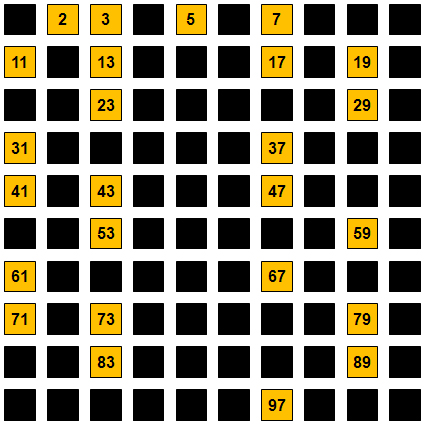
\epsfig{file=includes/images/primzahlen100.jpg, height=3in, width=3in}
		\caption{Primzahlen bis 100 Quelle: \cite{Mathe:Lexikon:SiebDesEratosthenes}}
		\label{ABBILDUNG_Primzahlen_100}
	\end{figure}
	
	\subsection{Effiziente Primzahltests} \label{Effiziente Primzahltests}
		Die in diesem Kapitel vorgestellten Algorithmen zum Erkennen von Primzahlen sind effiziente Algorithmen im Sinne der Komplexitätsklasse P und im Gegensatz zum fermatschen Test nicht anfällig für starke Pseudoprimzahlen. Dennoch unterscheiden sich die beiden vorgestellten Verfahren deutlich voneinander. Neben der Funktionsweise wird auch die Laufzeit gegenübergestellt.
		
		\subsubsection{Miller-Rabin-Test}
		 Der Miller-Rabin-Test ist ein probabilistischer Primzahltest und gehört zu den Montecarlo- Algorithmen. Im Gegensatz zum fermatschen Primzahltest ist der Miller-Rabin-Test nicht so anfällig für Carmichaelzahlen.
		
		\begin{comment}
		Wichtig: wegen +-1
		
				Ein interessanter Aspekt des Satzes von Fermat ist folgender: Sei p eine ungerade
				Primzahl und a zu p teilerfremd. Dann gilt (a(p−1)/2)2 ≡ 1 mod p. Da die Gleichung
				x2 = 1 im Körper Fp nur die Lösungen x = ±1 hat, folgt also a(p−1)/2 ≡ ±1 mod p
		\end{comment}	
		\subsubsection{AKS-Test}
		Der AKS-TestEntwickelt von ... ist ein deterministischer in polinimieller Zeit durchführbarer Primzahltest. 
		
		
		